\documentclass[12pt,a4paper]{article}
\usepackage[utf8]{}
\usepackage[T1]{fontenc}
\title{Révision français}
\author{Louis Hardy}
\date{Mai 2019}

\renewcommand{\baselinestretch}{0.2}

\setlength{\hoffset}{-18pt}         
\setlength{\oddsidemargin}{0pt} % Marge gauche sur pages impaires
\setlength{\evensidemargin}{0pt} % Marge gauche sur pages paires
\setlength{\marginparwidth}{54pt} % Largeur de note dans la marge
\setlength{\textwidth}{481pt} % Largeur de la zone de texte (17cm)
\setlength{\voffset}{-18pt} % Bon pour DOS
\setlength{\marginparsep}{7pt} % Séparation de la marge
\setlength{\topmargin}{0pt} % Pas de marge en haut
\setlength{\headheight}{13pt} % Haut de page
\setlength{\headsep}{4pt} % Entre le haut de page et le texte
\setlength{\footskip}{27pt} % Bas de page + séparation
\setlength{\textheight}{720pt} % Hauteur de la zone de texte (25cm)

\usepackage{natbib}
\usepackage{graphicx}

\begin{document}

\section*{Springboard - Blog}
https://www.springboard.com/blog/machine-learning-interview-questions/ \\
\begin{enumerate}
   \item Bias vs Variance
   \begin{itemize}
     \item \textbf{Bias} is due to erroneus or overly simplistic assumptions in learning algorithm
     \item Usually underfitting your data
     \item \textbf{Variance} typically due to too much complexity in learning algorithm
     \item Makes the model sensitive to high degrees of variation in training data. 
     \item Too much noise from training data
     \item If you make data more complex and add more variables, you'll lose bias but gain variance. 
   \end{itemize}
   \item Supervised vs Unsupervised learning
   \begin{itemize}
       \item Supervised requires labeled data. Unsupervised does not. 
    \end{itemize}
    \item How is KNN different from k-means clustering?
    \begin{itemize}
        \item KNN is a supervised classification algorithm. 
        \item K-means clustering is unsupervised. 
        \item Works very similarly
        \item KNN required labelled data 
        \item K means clustering requires only a set of unlabeled point and a threshold
        \item The algorithm will gradually \textit{learn} how to cluster them by computing mean of the 
              distance between different points.
    \end{itemize}
    \item How does a ROC curve work
    \begin{itemize}
      \item graphical representation of constrast between true and false positive rate at various 
            threholds. 
      \item Used as a proxy for trade-off between sensitivity of model (true positive) vs the 
            fall-out or probability it will trigger a false alarm (false positives)
      \item Think about recall and precision in this case.
        \begin{itemize}
          \item \textit{ex. } You'd have perfect recall (there are actually 10 apples, and you 
                predicted there would be 10) but $66.7\%$ precision because out of the 15 events 
                you precited, only 10 (the apples) are correct.
        \end{itemize}
    \end{itemize}
    \item  Baye's Theorem?
    \begin{itemize}
      \item $$P(A|B) = \frac{P(B|A)P(A)}{P(B)}$$
      \item Leads to a branch of ML called Naive Bayes classifier
    \end{itemize}
    \item Why is "Naive" Bayes naive?
    \begin{itemize}
      \item Used a lot in text mining
      \item It's naive because it makes an assumption that is virtually impossible in real-life data. 
      \begin{itemize}
        \item conditional probability is calculated as the pure product of the individial probabilities of components.
        \item This implies absolute independence of features - condition probably never met in real life.
      \end{itemize}
      \item Anohter way put, if a Naive Bayes classifier figured that you liked pickles and ice-cream 
            would probably naively recommend you a pickle ice-cream.
    \end{itemize}
    \item Difference between L1 and L2 regularization
    \begin{itemize} % 7
      \item Regularization helps solve over-fitting problems in ML
      \item Simple model will be very poor generalization of data. 
      \item Complex model may not perform well in test due to over-fitting.
      \item Regulatization refers to adding a penalty term to objective function and control model complexity using 
            that penalty term. 
      \item Ridge regression used $L_2$ norm for regularization.
      \begin{itemize}
        \item Ridge regression is used to analyze techniques that suffer from multicollinearity.
        \item When multicollinearity occurs, least squares estimates are unbiased, but variances are large so they might
              be far from true value.
      \end{itemize}
      \item L2 forces weights to be small but does not make them zero 
            and does non sparse solution
      \item Lasso regression uses L1 regression
      \begin{itemize}
        \item Type of linear regression that uses shrinkage. 
        \item Shrinkage is where data values are \textit{shrunk} towards 
              a central point, like the mean.
        \item Creates simple sparse models (models with fewer parameters)
      \end{itemize}
      \item Main difference between L1 and L2 is the difference between the constraint
            region. 
    \end{itemize}
    \item Favorite algorithm
    \begin{itemize}
      \item Optical flow is pattern of apparent motion of objects, surfaces, 
            and edges caused by the relative motion between an observer and 
            a scene. 
      \item Optical flow methods try to calculate motion between between two 
            images which are taken at times $t$ and $t + \Delta t$ at every
            voxel position. 
      \item This sort of method are called differential since they are based 
            on local Taylor Series.
      \item They use partial derivatives with respect to spatial and temporal 
            coordinates. 
    \end{itemize}
    \item Difference between Type I and Type II error?
    \begin{itemize}
      \item Type I error is rejection of true null hypothesis ("false" positive)
      \item Type II error is not rejective the false null hypothesis 
    \end{itemize}
    \item Fourier Transform
    \begin{itemize}
      \item Converts signal from time to frequency domain
      \item Decomposes generic function into a superposition of symmetric 
            function.
    \end{itemize}
    \item Probability vs Likelihood [Need to expand]
    \begin{itemize}
      \item Probability attaches to possible results
      \item Likelihood attaches to hypothesis
    \end{itemize}
    \item Difference between generative and discriminative model
    \begin{itemize}
      \item Generative model will learn categories of data
      \item Discriminative will simply learn the different categories 
            of data.
      \item Discriminative will generally outperform generative models 
            on classification tasks.
    \end{itemize}
    \item What CV technique would you use on time-series dataset
    \begin{itemize}
      \item Time series is not randomly distributed but 
            but chronologically ordered.
      \item Forward chaining is one way of doing this
      \begin{itemize}
        \item In time series CV each day is a test data and the 
              previous day's data is the training set.  \\
        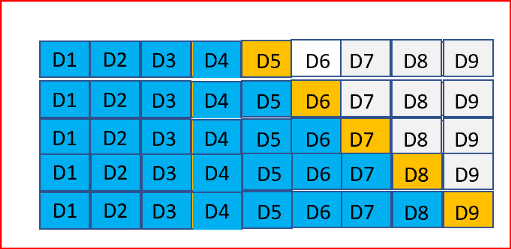
\includegraphics[width=10cm]{forward_chaining.png} \\
        \item We start training the model with a minimum number 
              of observations and use the next day's data to 
              test the model and we keep moving through the data 
              set. 
      \end{itemize}
    \end{itemize}
  \item Decision tree pruned
  \begin{itemize}
    \item Pruning is what happens in decision trees when branches 
          that have weak predictive power are remove.
    \item This reduces model complexity and increases predictive 
          accuracy of a decision tree model. 
    \item Reduced error pruning is simplest version
    \begin{itemize}
      \item replace each
      \item if it doesn't decrease predictive accuracy, keep it 
            pruned.
    \end{itemize}
  \item What is more important to you - model accuracy or model 
        performance?
    \begin{itemize}
      \item Accuracy paradox
      \item A simple model may have a high level of accuracy but 
            be too crude to be useful
      \item If you have a large dataset to detect fraud and majority 
            of it are not-fraud data points, the probability of the 
            model detecting fraud is a lot lower. 
      \item model designed to find fraud that asserted there was no 
            fraud at all. 
    \end{itemize}
  \end{itemize}
  \item F1 score
  \begin{itemize}
    \item F1 score is measure of model's performance
    \item Weighted average of precision and recall of a 
          model, with results tending to 1 being the best 
          and those tending to 0 being the worst.
    \item Used in classification tests where true negatives 
          don't matter much. 
  \end{itemize}
  \item How to handle an imbalanced dataset?
  \begin{itemize}
    \item Imbalanced dataset is when 90\% of the data is in one 
          class
    \item this accuracy can lead to a skewed of one prediction class
    \item These are ways to get over the hump
    \begin{itemize}
      \item Collect more data to even the imbalances in the dataset
      \item Resample dataset to correct for imbalances
      \item Try a different algorithm on your dataset
    \end{itemize}
  \end{itemize}
  \item When should you use classification over regression?
  \begin{itemize}
    \item Classification produces discrete values. 
    \item Regression is continuous
    \item Seeing if a name is male or female vs how correlated 
          they were with male and female names.
  \end{itemize}
  \item Example where ensemble techniques might be useful
  \begin{itemize}
    \item Ensemble technique uses a combination of learning 
          algorithms to optimize better predictive performance. 
    \item Typically reduces overfitting in models and and makes model 
          more robust (unlikely to be influence by small changes in 
          the training data).
    \item \textit{ex. } bagging
  \end{itemize}
\end{enumerate}
\noindent\hrulefill

\section*{Building a recommendation system}
\begin{enumerate}
  \item Simply put, the engine computes the co-occurrence matrix
        from a history matrix of events and actions. 
  \item Then, we have to apply statistics to filter out the 
        sufficiently anomalous signals to be interesting as a 
        recommendation.
  \item We need to be able to extract \textbf{relevant indicators} 
        from the co-occurrence matrix. This is what makes a good 
        recommendation system.
  \item Creating an item-to-item indicator matrix is called an 
        \textbf{item-item model}. Another one is a \textbf{user-item model}.
  \item   
\end{enumerate}

\end{document}